%!TEX root = ../../../report.tex
\section{3D printing} % (fold)
\label{sec:3d_printing}
The parts modeled for the project and shown in section \ref{sub:computer_aided_design}, have been printed using Fused Filament Fabrication (FFF).
The 3D printer used is a M Prime One \footnote{https://github.com/M-Prime/M\_Prime\_One} with a 0.4 mm noozle.
All the parts have been printed at 0.2 mm layer height.

The use of this technology is justify by the fact that makes the iterative process between design and manufacturing both fast and cheap. \todo{Fast and low-cost prototyping}
All the parts have been individually adjusted until the clearances have been as expected.
Furthermore, this enable the user not only to replicate the parts with out any considered extra cost, but allows the robot to be easily replicated in other places.

When manufacturing, some of the parts have needed material support.
\todo{Why the material support? Tell how you've managed to print the most complex stuff}
The figure \ref{fig:photo_material_support} depicts two feet, one with material support and the other with it removed.
In the figure \ref{fig:photo_3d_printed} a detail of actual parts 3D printed and assembled in the robot are shown.

\begin{figure}[ht]
    \centering
    \begin{subfigure}[b]{0.49\textwidth}
        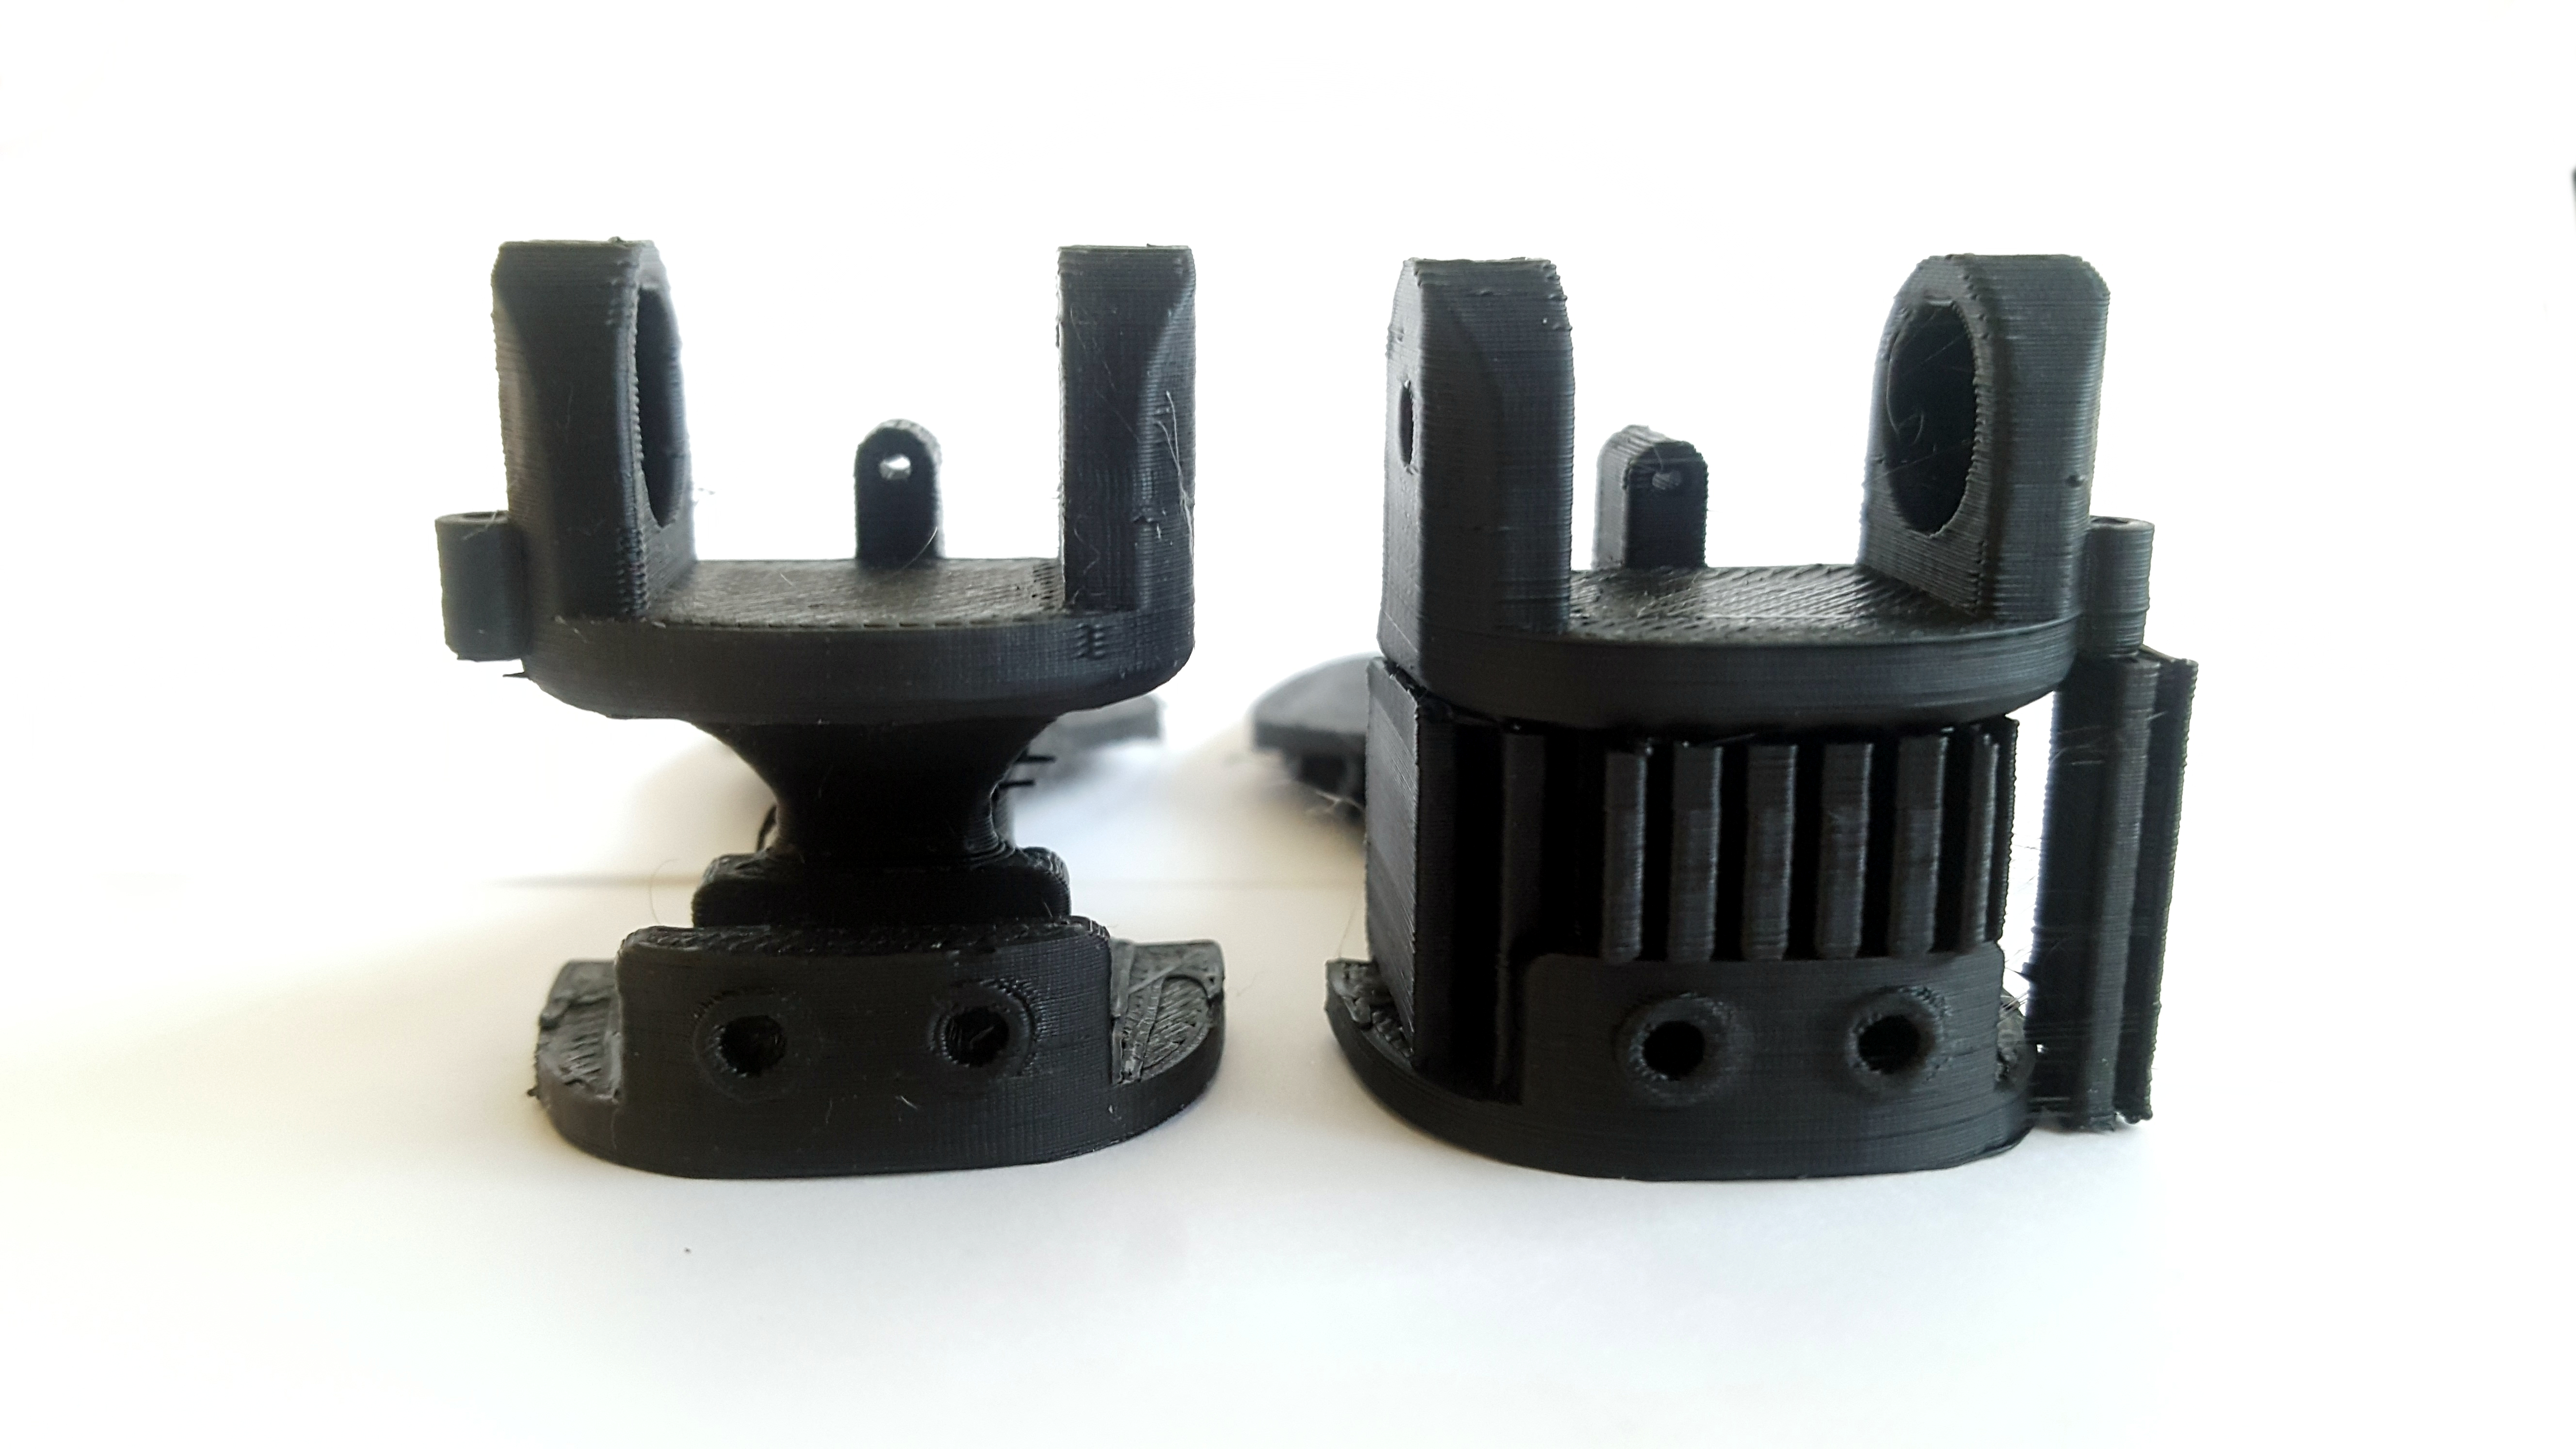
\includegraphics[width=\textwidth]{figures/photo_material_support.jpg}
        \caption{Feet with and without material support}
        \label{fig:photo_material_support}
    \end{subfigure}
    \begin{subfigure}[b]{0.49\textwidth}
        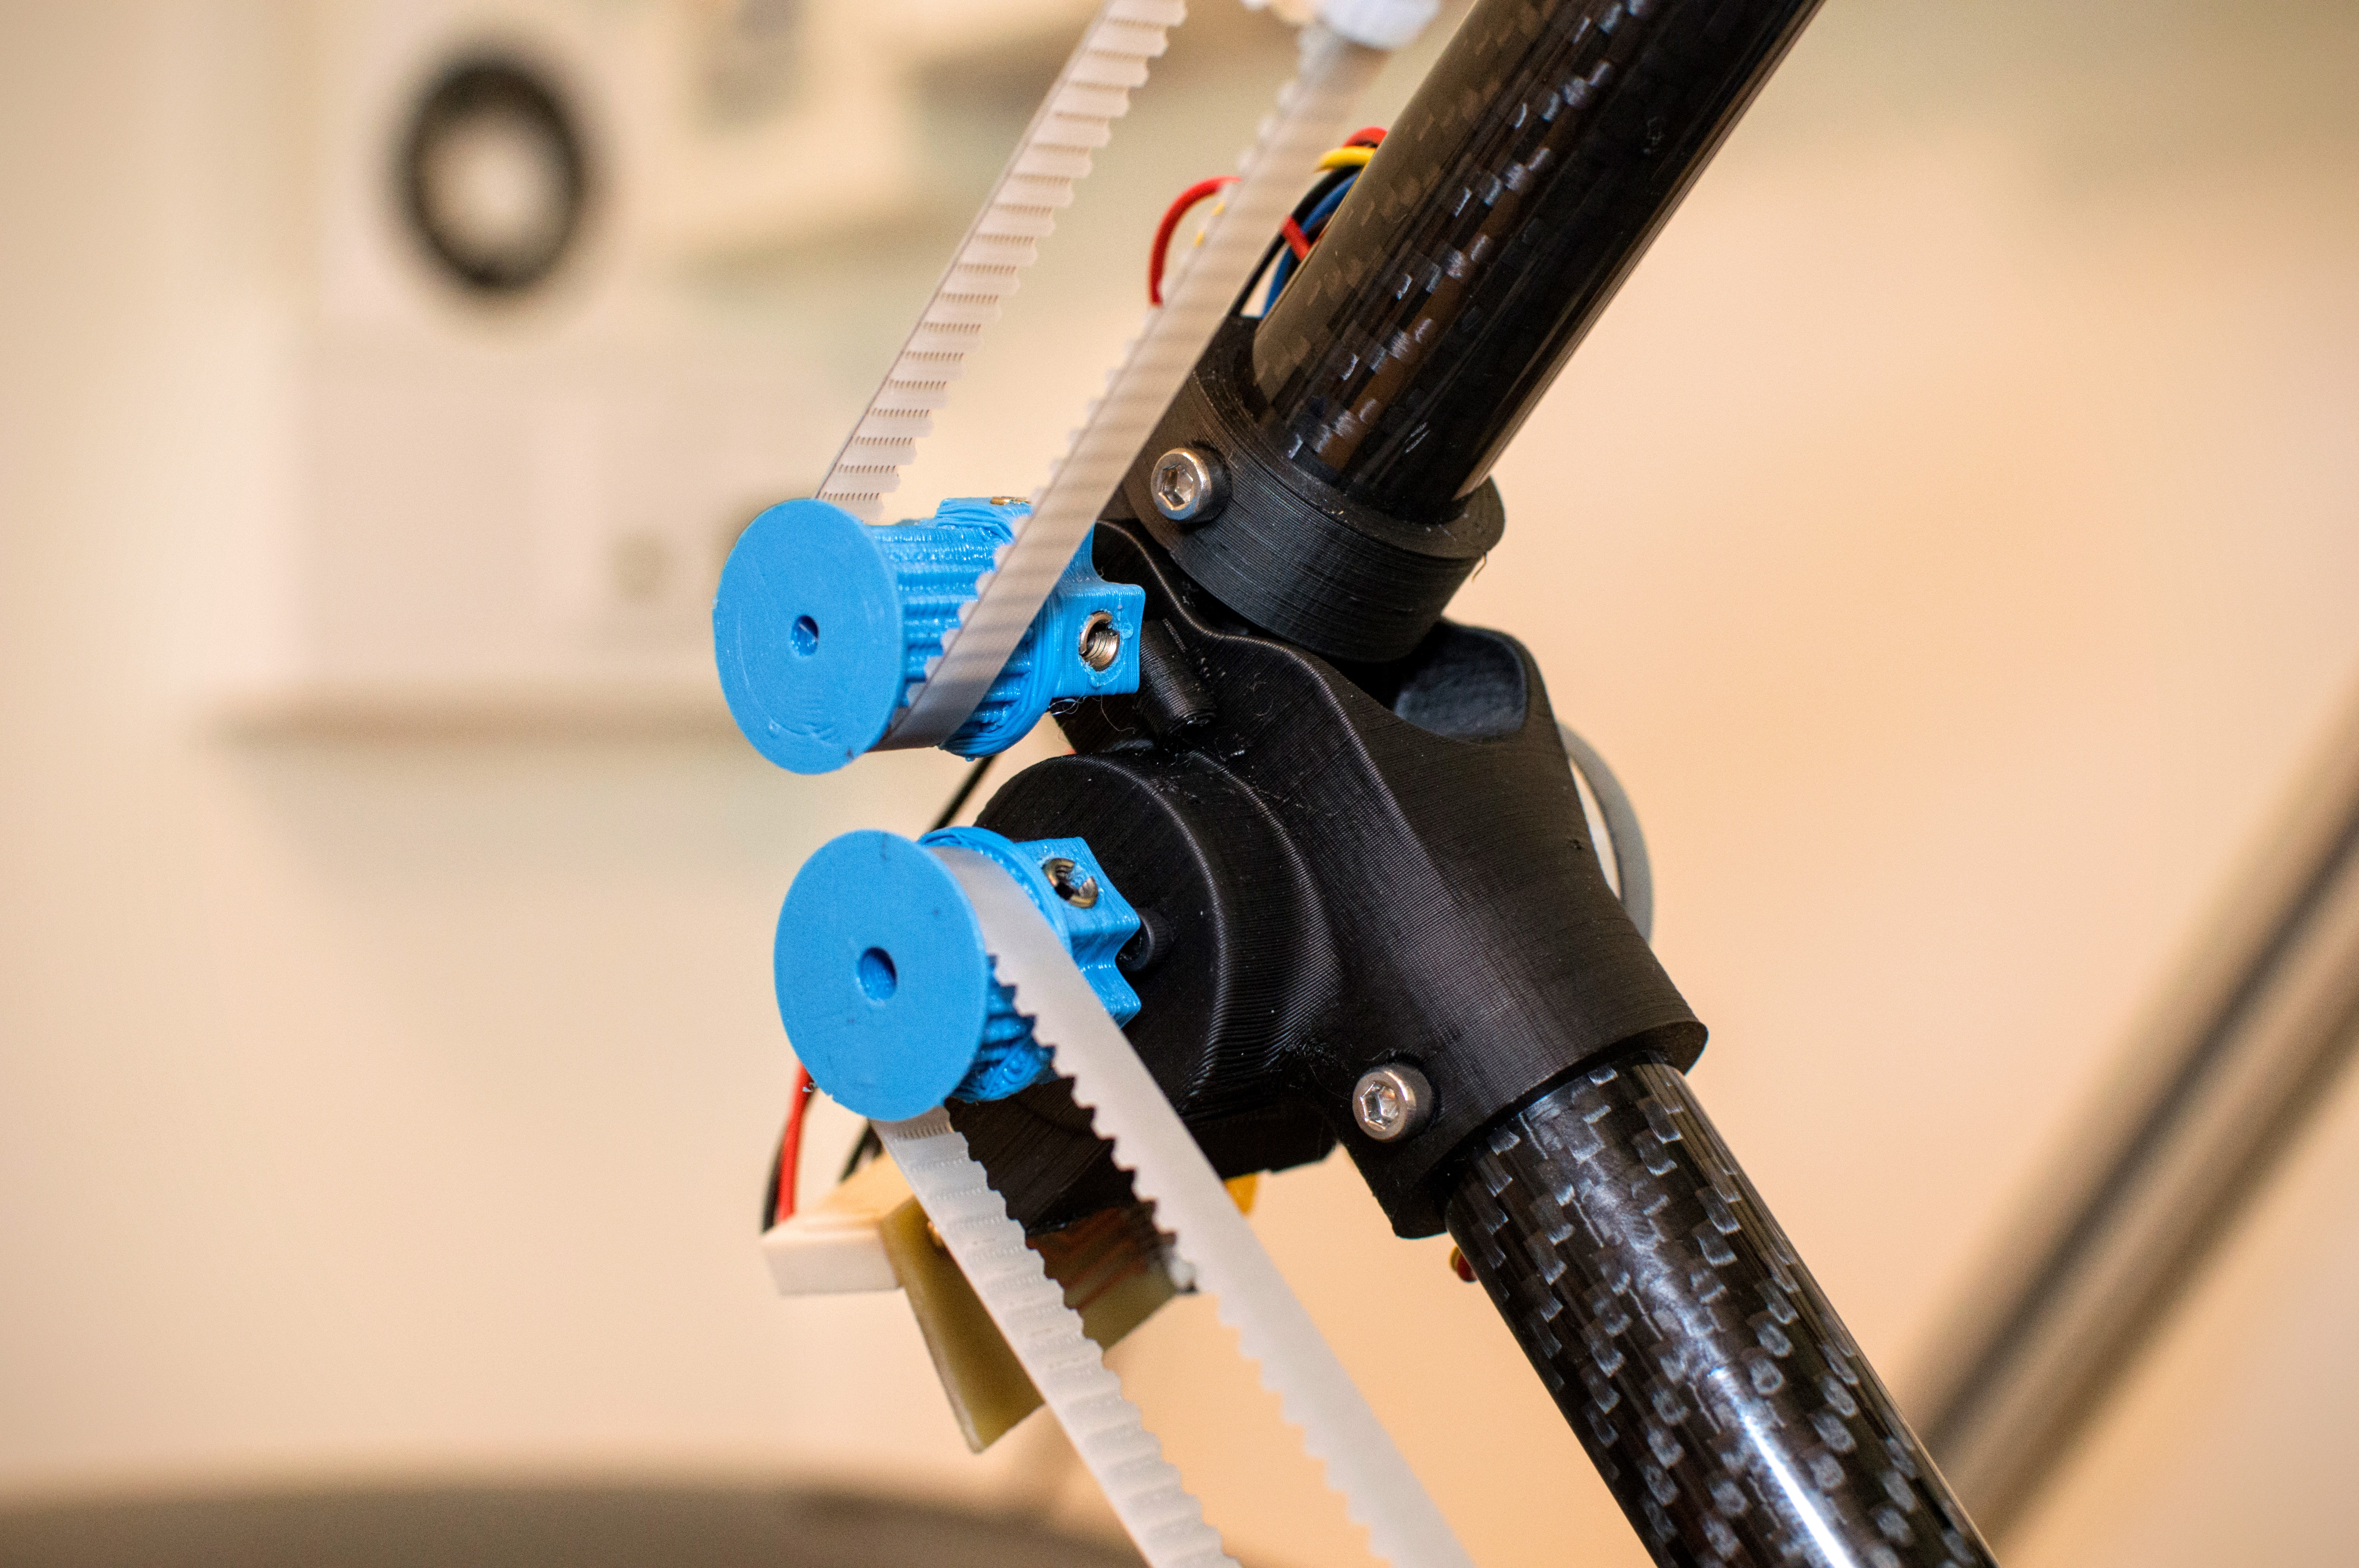
\includegraphics[width=\textwidth]{figures/photo_3d_printed.jpg}
        \caption{Detail of 3D printed parts assembled}
        \label{fig:photo_3d_printed}
    \end{subfigure}
\end{figure}

  \subsection{Arc compensation} % (fold)
  \label{sub:arc_compensation}
  For the CAD models of the 3D printed parts, the clearances of the internal holes have been adjusted following \cite{arc_compensation}.
  The undersizing of internal holes is a common problem in this sort of technology due to the lack of information of the common-used exporting format: the STL.
  This only contains the 3D model expressed as a set of external triangles, which difficult the correction of malformations inherent to the technology.

  In the case of the Fused Filament Fabrication (FFF), the material is extruded equally in both sides of the arc, as shown in \ref{fig:arc_compensation}. 
  However, in the side of the smaller curve, less material is needed.
  This correction can be calculated with:

  \todo{Label and reference the equations}
  $$ r=\frac{t+\sqrt{t^2+4R^2}}{2}$$

  being:
  \begin{enumerate}
    \item t: noozle diameter
    \item R: desired internal hole radius
    \item r: corrected radius
  \end{enumerate}
  As an example, Klee suggests an internal hole of 4.4 mm in the case of the selected nuts \cite{klee}. Thus, the diameter in the CAD model has been adjusted for this data and a noozle of 0.4 mm. The result is then:
  $$ d=2r=\frac{t+\sqrt{t^2+4R^2}}{2}=0.4+\sqrt{0.4^2+4*2.2^2}=4.81$$

  \begin{figure}[tb]
    \centering
    \includegraphics[width=0.5\textwidth]{figures/Arc-compensation}
    \caption{Technical representation of the generated arc when using FFF technology}
    \label{fig:arc_compensation}
  \end{figure}
  % subsection arc_compensation (end)

% section 3d_printing (end)